\documentclass[a4paper,dutch]{article}
\usepackage{babel}
\usepackage{pxfonts}
\usepackage{listings}
\usepackage{answers}
\usepackage{tikz}
\usepackage{hyperref}
\usepackage{cleveref}

\newtheorem{exercise}{Oefening}[section]
\Newassociation{solution}{Oplossing}{answers}


\lstdefinelanguage{MyJava}[]{java}{
  escapeinside=\`\`,%
  basicstyle={\ttfamily\small},%
  keywordstyle={\ttfamily\bfseries},%
  commentstyle={\it},%
  frame=lines,%
  showstringspaces=false,%
}

\newcommand{\code}[2][]{
  \lstinputlisting[language=MyJava,#1]{#2}
}


\begin{document}

\Opensolutionfile{answers}

\section{Methodes van de klasse {\tt Hint}}
E\'en van de aspecten van het spel galgje is dat er sprake is van een te raden woord
waarvan de letters stapsgewijs verschijnen.
We kunnen de verantwoordelijkheid
voor deze functionaliteit toekennen aan een klasse, dewelke we {\tt Hint} zullen noemen.
Eeh {\tt Hint}-object moet dus bijhouden wat het te raden woord is is tezamen met welke letters ervan zichtbaar zijn.
Een mogelijk gebruik van {\tt Hint} ziet er als volgt uit:
\code{hint-interaction.java}

\begin{exercise}
Welk datatype gebruiken we om een woord voor te stellen?
\begin{solution}
\tt String
\end{solution}
\end{exercise}

\begin{exercise}\label{exercise:field}
Welk datatype gebruiken we om voor te stellen of een letter al dan niet zichtbaar is?
\begin{solution}
\tt boolean
\end{solution}
\end{exercise}

\begin{exercise}
Een {\tt Hint}-object moet onthouden welk woord er geraden moet worden. Hoe kunnen we hiervoor zorgen?
\begin{solution}
Veld en constructor als volgt:
\code{hint-field-constructor.java}
\end{solution}
\end{exercise}

We moeten aan een {\tt Hint}-object kunnen vragen om een bepaalde letter zichtbaar te maken.
Deze methode moet tevens weten te zeggen of de gegeven letter voorkwam of niet (indien niet
moet er immers een extra lichaamsdeel bijgetekend worden).

\begin{exercise}
Stel dat we deze methode {\tt reveal} noemen, wat is de signatuur?
\begin{center}
  \rule{2cm}{.5pt} {\tt reveal(}\rule{4cm}{.5pt}{\tt)}
\end{center}
\begin{solution}
\tt boolean reveal(char letter)
\end{solution}
\end{exercise}

\begin{exercise}
We moeten kunnen weten of het ganse woord zichtbaar is. Wat is de signatuur?
\begin{center}
  \rule{2cm}{.5pt} {\tt isFullyRevealed(}\rule{4cm}{.5pt}{\tt)}
\end{center}
\begin{solution}
\tt boolean isFullyRevealed()
\end{solution}
\end{exercise}

\begin{exercise}
Uiteindelijk moeten we ook de hint kunnen ``tonen''. We noemen deze methode {\tt show}.
Wat is de signatuur van deze methode?
\begin{center}
  \rule{2cm}{.5pt} {\tt show(}\rule{4cm}{.5pt}{\tt)}
\end{center}
\begin{solution}
\tt String show()
\end{solution}
\end{exercise}

\section{Methodes hulpklasse {\tt HintBox}}
We kunnen {\tt Hint} op veel manieren implementeren. Voor deze oefening
voeren we een hulpklasse {\tt HintBox} in. Een {\tt HintBox}-object is gelijkaardig aan {\tt Hint} maar zal instaan
voor slechts \'e\'en enkele letter:
\begin{itemize}
  \item De {\tt HintBox} moet weten welke letter het bevat.
  \item De {\tt HintBox} moet bijhouden of de letter geraden werd of niet.
\end{itemize}
Een {\tt Hint} zal dus intern een lijst bijhouden van {\tt HintBox}-objecten,
\'e\'en voor elke letter van het te raden woord. 
\begin{center}
  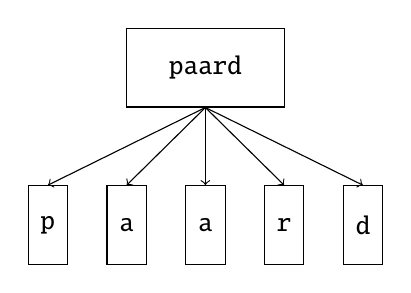
\begin{tikzpicture}
    \node[draw,minimum width=2cm,minimum height=1cm] (Hint) at (2,1) {\tt paard};
    \foreach \x/\c in {0/p,1/a,2/a,3/r,4/d} {
      \node[draw,minimum width=.5cm,minimum height=1cm] (box \x) at (\x,-1) {\tt\c};
      \draw[->] (Hint.south) -- (box \x.north);
    }
  \end{tikzpicture}
\end{center}
{\tt Hint} zal in zijn eigen methodes
beroep doen op de methodes van {\tt HintBox}. Een mogelijke interactie gaat als volgt:
\code{hintbox-interaction.java}
Merk op dat {\tt HintBox} methodes bevat met dezelfde naam als {\tt Hint}:
voor zover Java weet hebben deze, doordat de methodes in verschillende klassen zitten,
niets met elkaar te maken. 
Gezien beide klassen gelijkaardige
functionaliteit aanbieden, is het ook maar normaal dat ze gelijkaardige methodes bevatten.
We gaan nu na welke functionaliteit een {\tt HintBox} moet aanbieden
opdat {\tt Hint} zijn werk kan doen.

\begin{exercise}
Wat is het type voor \'e\'en enkele letter?
\begin{solution}
\tt char
\end{solution}
\end{exercise}

Een {\tt Hint}-object biedt een {\tt reveal}-methode aan, zoals eerder besproken.
Het zichtbaar maken van een letter houdt in ons design in dat we aan
elk van de {\tt HintBox}-objecten vragen diezelfde letter zichtbaar te maken.

\begin{center}
  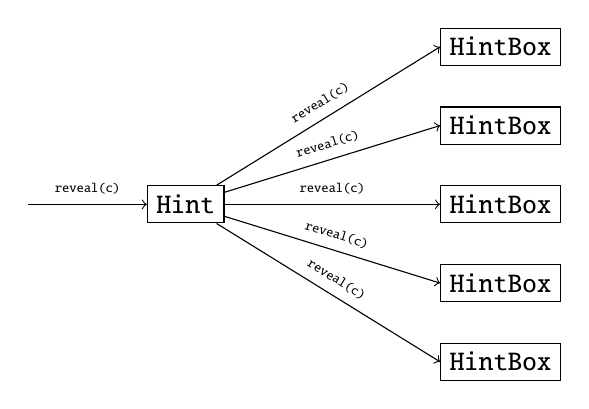
\begin{tikzpicture}
    \node[draw] (Hint) at (0,0) {\tt Hint};
    \foreach \y in {-2,...,2} {
      \node[draw] (HintBox \y) at (4,\y) {\tt HintBox};
      \draw[->] (Hint) -- (HintBox \y.west) node [midway,sloped,above] {\tt\tiny reveal(c)};
    }
    \draw[->] (-2,0) -- (Hint.west) node [midway,anchor=south] {\tt\tiny reveal(c)};
  \end{tikzpicture}
\end{center}

\begin{exercise}
Wat is de signatuur van {\tt HintBox.reveal}? Denk eraan dat de methode ook
een manier moet hebben om aan te geven of de letter ``juist'' was (d.i.\ om te weten
of er een lichaamsdeel bijgetekend moet worden of niet.)
\begin{center}
  \rule{2cm}{.5pt} {\tt reveal(}\rule{4cm}{.5pt}{\tt)}
\end{center}
\begin{solution}
\tt boolean reveal(char letter)
\end{solution}
\end{exercise}

De informatie of een letter zichtbaar is of niet zit in {\tt HintBox}. De klasse {\tt Hint}
heeft deze informatie nodig om zijn eigen methode {\tt isFullyRevealed()} te kunnen implementeren.
{\tt Hint} moet dus aan een {\tt HintBox}-object kunnen vragen of de letter zichtbaar is.
Hiervoor voeren we een methode {\tt isRevealed()} in in de klasse {\tt HintBox}.
{\tt Hint} zal dan in zijn implementatie van {\tt isFullyRevealed()} aan elke {\tt HintBox} vragen
of zijn letter zichtbaar is; indien ze allemaal positief antwoorden, moet {\tt isFullyRevealed} zelf ook
{\tt true} teruggeven.

\begin{center}
  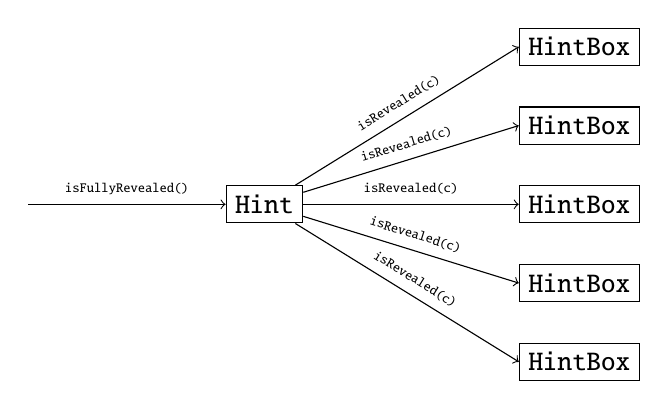
\begin{tikzpicture}
    \node[draw] (Hint) at (0,0) {\tt Hint};
    \foreach \y in {-2,...,2} {
      \node[draw] (HintBox \y) at (4,\y) {\tt HintBox};
      \draw[->] (Hint) -- (HintBox \y.west) node [midway,sloped,above] {\tt\tiny isRevealed(c)};
    }
    \draw[->] (-3,0) -- (Hint.west) node [midway,anchor=south] {\tt\tiny isFullyRevealed()};
  \end{tikzpicture}
\end{center}


\begin{exercise}
Wat is de signatuur van {\tt HintBox.isRevealed}?
\begin{center}
  \rule{2cm}{.5pt} {\tt isRevealed(}\rule{4cm}{.5pt}{\tt)}
\end{center}
\begin{solution}
\tt boolean isRevealed()
\end{solution}
\end{exercise}

Uiteindelijk moet {\tt HintBox} ook een eigen {\tt show} methode hebben. Indien
de letter zichtbaar is, moet deze deze letter teruggeven als resultaat;
in het andere geval \verb'"_"'.

\begin{exercise}
Wat is de signatuur van {\tt HintBox.show}?
\begin{center}
  \rule{2cm}{.5pt} {\tt show(}\rule{4cm}{.5pt}{\tt)}
\end{center}
\begin{solution}
\tt String show()
\end{solution}
\end{exercise}

\section{Implementatie van {\tt HintBox}}
We beginnen met de implementatie van de eenvoudigste klasse, nl.\ {\tt HintBox}.
Zoals eerder vermeld, houdt deze twee dingen bij: de te raden letter, en of de letter
zichtbaar is of niet. Hiervoor zijn dus duidelijk velden nodig.

\begin{exercise}
Welke twee velden heeft {\tt HintBox} nodig?
\begin{solution}
Een veld {\tt char letter} en een veld {\tt boolean isRevealed}.
\end{solution}
\end{exercise}

Na het defini\"eren van velden implementeren we vaak de constructor.
We stellen ons de vraag wat een {\tt HintBox} nodig heeft om zichzelf
te initialiseren.

\begin{exercise}
Welke parameters krijgt de constructor binnen,
wetende dat een letter in het spel galgje standaard verborgen is.
Implementeer de constructor.
\begin{solution}
Onvolledige implementatie van de klasse:
\code{hintbox-constructor.java}
\end{solution}
\end{exercise}

We voegen nu \'e\'en na \'e\'en de methodes toe die we in de vorige paragraaf bespraken.
We beginnen met {\tt reveal(c)}: deze methode moet, indien {\tt c} gelijk is aan de letter
die in de {\tt HintBox} steekt, de zichtbaarheid op {\tt true} zetten.

\begin{exercise}
Implementeer {\tt HintBox.reveal}.
\begin{solution}
In de klasse {\tt HintBox}:
\code{hintbox-reveal.java}
\end{solution}
\end{exercise}

\begin{exercise}
Implementeer {\tt HintBox.isRevealed}.
\begin{solution}
In de klasse {\tt HintBox}:
\code{hintbox-isrevealed.java}
\end{solution}
\end{exercise}

\begin{exercise}
Implementeer {\tt HintBox.show}. Zoals in de vorige paragraaf beschreven moet deze ofwel
de letter ofwel \verb'"_"' teruggeven, naargelang de zichtbaarheid.
\begin{solution}
In de klasse {\tt HintBox}:
\code{hintbox-show.java}
\end{solution}
\end{exercise}

\section{Implementatie van {\tt Hint}}
We schakelen over naar de klasse {\tt Hint}. In \cref{exercise:field} waren we
tot de conclusie gekomen dat {\tt Hint} een veld {\tt String word} moest
bevatten om het te raden woord te kunnen onthouden; blijkt
nu dat dit niet het geval is, omdat dezelfde informatie
zal bijgehouden worden door {\tt HintBox}-objecten.

\begin{exercise}
Een {\tt Hint}-object bevat \'e\'en {\tt HintBox} per letter. Wat is hiervoor nodig?
\begin{solution}
Een veld {\tt HintBox[] hintBoxes}.
\end{solution}
\end{exercise}

Om een {\tt Hint}-object aan te maken, geven we een woord aan de constructor.
Met {\tt String.charAt} kan deze opvragen uit welke letters deze opgebouwd is
en voor elke letter een overeenkomstige {\tt HintBox} maken.
\begin{exercise}
Schrijf de constructor van de klasse {\tt Hint}.
\begin{solution}
In de klasse {\tt Hint}:
\code{hint-constructor.java}
\end{solution}
\end{exercise}

\begin{exercise}
Schrijf de methode {\tt reveal}: gegeven een letter moet de methode deze letter
doorgeven aan elke {\tt HintBox}.
\begin{solution}
In de klasse {\tt Hint}:
\code{hint-reveal.java}
\end{solution}
\end{exercise}

\begin{exercise}
Schrijf de methode {\tt isFullyRevealed}.
\begin{solution}
In de klasse {\tt Hint}:
\code{hint-isfullyrevealed.java}
\end{solution}
\end{exercise}

\begin{exercise}
Schrijf de methode {\tt show}. Deze moet de {\tt show}-methode van elke {\tt HintBox}
oproepen en de resultaten aan elkaar rijgen, maar telkens met een spatie ertussen.
\begin{solution}
In de klasse {\tt Hint}:
\code{hint-show.java}
\end{solution}
\end{exercise}

\Closesolutionfile{answers}
\clearpage
\section{Oplossingen}
\begin{Oplossing}{8.1.1}
De elementen zullen van groot naar klein gesorteerd worden.
\end{Oplossing}
\begin{Oplossing}{8.1.2}
Indien de rij twee gelijke elementen bevatten, zullen deze constant verwisseld
worden en eindigt het algoritme nooit.
\end{Oplossing}
\begin{Oplossing}{8.1.3}
\inlinecode{i > 0} geeft exact hetzelfde als \inlinecode{i >= 0} vermits
\inlinecode{bubbleSortPass} nooit \inlinecode{0}
kan teruggeven: ofwel worden er geen elementen aangepast en geeft de functie \inlinecode{-1}
terug, ofwel wordt \inlinecode{i+1} teruggegeven waarbij \inlinecode{i} minimaal gelijk is aan \inlinecode{0}.
Met andere woorden, indien het element met index \inlinecode{0} wordt verplaatst, \emph{moet} ook
het element met index \inlinecode{1} zijn betrokken geweest. Vermits de index van het laatste verplaatste element
(d.i.\ dat met de hoogste index) moet teruggegeven worden, betekent dit dat \inlinecode{1} het resultaat moet zijn
(of een hogere index indien er nog andere elementen verwisseld werden).
\end{Oplossing}
\begin{Oplossing}{8.2.1}
Het resultaat blijft hetzelfde. Het geval waarbij \inlinecode{i} gelijk is aan
\inlinecode{0} komt overeen met het invoegen van een element in een lege rij.
Vermits hiervoor in ons geval niets hoeft te gebeuren, kunnen we deze stap gewoon overslaan.
In \cref{example:sorteer:insertion} kwamen we dit ook tegen: het invoegen
van 6 benodigde geen verwisselingen.
\end{Oplossing}
\begin{Oplossing}{8.2.2}
Dit doe je best niet vermits je het risico loopt om, indien \inlinecode{i == 0},
\inlinecode{rij[-1]} met \inlinecode{rij[0]} te vergelijken.
Een conjunctie (\inlinecode{&&}) wordt van links naar rechts uitgevoerd:
indien de linkervoorwaarde faalt, zal de rechtervoorwaarde niet ge\"evalueerd worden.
Eerst nakijken of \inlinecode{i-1 >= 0} verhindert dus dat \inlinecode{rij[i-1] > rij[i]}
wordt uitgevoerd indien \inlinecode{i} niet groter is dan \inlinecode{0}.

Terzijde: hoewel het gedrag
van zulke code wel gedefinieerd is in JavaScript (\inlinecode{rij[-1]} zal de waarde \inlinecode{undefined}
opleveren) en ironisch genoeg de code uiteindelijk zelfs zal werken (je kan zelfs
\inlinecode{i-1 >= 0} weglaten!), moet je JavaScript al h\'e\'el goed kennen
om op zulk gedrag te kunnen steunen teneinde correct werkende algoritmen te schrijven.
De bedoeling van deze cursus om de algoritmen te begrijpen en te kunnen implementeren,
en niet de gekheden en frivoliteiten van JavaScript te leren benutten;
indien je code steunt op zulke taalspecifieke details, zal het dan ook als fout beschouwd worden.
We willen dus dat je code weldegelijk \emph{eerst} checkt dat \inlinecode{i-1 >= 0}.
\end{Oplossing}
\begin{Oplossing}{8.2.3}
Het algoritme geeft in dit geval \inlinecode{i} terug, wat in feite foutief is.
De functie \inlinecode{selectionSort} roept echter \inlinecode{zoekIndexMinimum}
op met \inlinecode{i <= imax} waardoor alles correct werkt. In principe zou
men echter \inlinecode{zoekIndexMinimum} robuuster moeten maken.
\end{Oplossing}
\begin{Oplossing}{8.2.4}
Het geval \inlinecode{i == rij.length - 1} betekent dit dat we aan het laatste
element toe zijn. De rode rechterdeelrij bevat dus slechts \'e\'en enkel element.
Het minimum hiervan vinden is triviaal: het is dat element zelf.
We zouden dus \inlinecode{minimumIndex == i} bekomen. Vervolgens zouden we
op \cref{line:sorteer:selection:swap} die element met zichzelf verwisselen,
wat geen effect heeft. Met andere woorden, het laatste element krijgen we ``gratis'':
het staat automatisch reeds op de juiste plaats in de rij.
\end{Oplossing}
\begin{Oplossing}{8.3.1}
\inlinecode{mergeSortRec} zal zichzelf nooit oproepen met \inlinecode{begin > einde},
maar \inlinecode{mergeSort} zal echter wel \inlinecode{mergeSortRec} kunnen oproepen
met \inlinecode{begin==0} en \inlinecode{einde==-1}: dit komt voor indien
men de lege rij wil sorteren. Hoewel dit wel een randgeval is, is het belangrijk
dat dit ook correct wordt afgehandeld.
\end{Oplossing}


\end{document}